\chapter{Rules of Schafkopf}
Schafkopf is a traditional four player trump card game that is played in the south of Germany.
The game is widely popular for being easy to learn but allowing for deep strategies.
Often it is played for small money stakes, but can also be enjoyed casually.
A hand of Schafkopf consist of eight tricks, and four hands make a round.
A game of Schafkopf consists therefore of multiple rounds, where the intial dealer position rotates
clockwise around the table after each hand.
In order to play a hand, players will bid between themselves for a game contract, creating either two teams of two or
two teams of one and three, and then play eight tricks with differing rules sets that depend on the winning bid.

\section{Cards}\label{sec:cards}
The Game of Schafkopf uses a 32 card bavarian deck, containing 4 suits with 8 ranks each.
Since the bavarian deck is comparable with a 52 french deck, where all ranks 2-6 are excluded, we also included the
corresponding English names for each suit and rank in the following tables.
The following tables is ordered descendingly by strength:
\newline
\begin{table}[h!]
    \centering
    \begin{tabular}{lll}
        \toprule
        Suit     & Short Hand & Corresponding French Suit \\
        \midrule
        Eichel   & E          & Clubs                     \\
        Gras     & G          & Spades                    \\
        Herz     & H          & Hearts                    \\
        Schellen & S          & Diamonds                  \\
        \bottomrule
    \end{tabular}
    \caption{The four suits of Schafkopf}
    \label{tab:suits}
\end{table}
\newline
Regardless of the contract each rank has a corresponding point value ranging from 11 to 0 points in discrete steps.
The total value of all 32 cards is therefore 120.
\newline
Table \ref{tab:cardsvalues} shows the order of ranks and their values.
\newline
\begin{table}[h!]
    \centering
    \begin{tabular}{llll}
        \toprule
        Rank  & Point Value & Short Hand & Corresponding French Rank \\
        \midrule
        Ass   & 11          & A          & Ace                       \\
        Zehn  & 10          & T          & Ten                       \\
        König & 4           & K          & King                      \\
        Ober  & 3           & O          & Queen                     \\
        Unter & 2           & U          & Jack                      \\
        9     & 0           & 9          & Nine                      \\
        8     & 0           & 8          & Eight                     \\
        7     & 0           & 7          & Seven                     \\
        \bottomrule
    \end{tabular}
    \caption{Card ranks of Schafkpopf and their point values}
    \label{tab:cardsvalues}
\end{table}
\newline
In order to refer to cards in the future we also included a short hand way of expressing suit and rank.
For example the Ten of Herz is TH and the Ober of Gras is OG.
A visual of all 32 cards in their traditional representation can be seen in Figure \ref{fig:32cards}
\begin{figure}[h!]
    \centering
    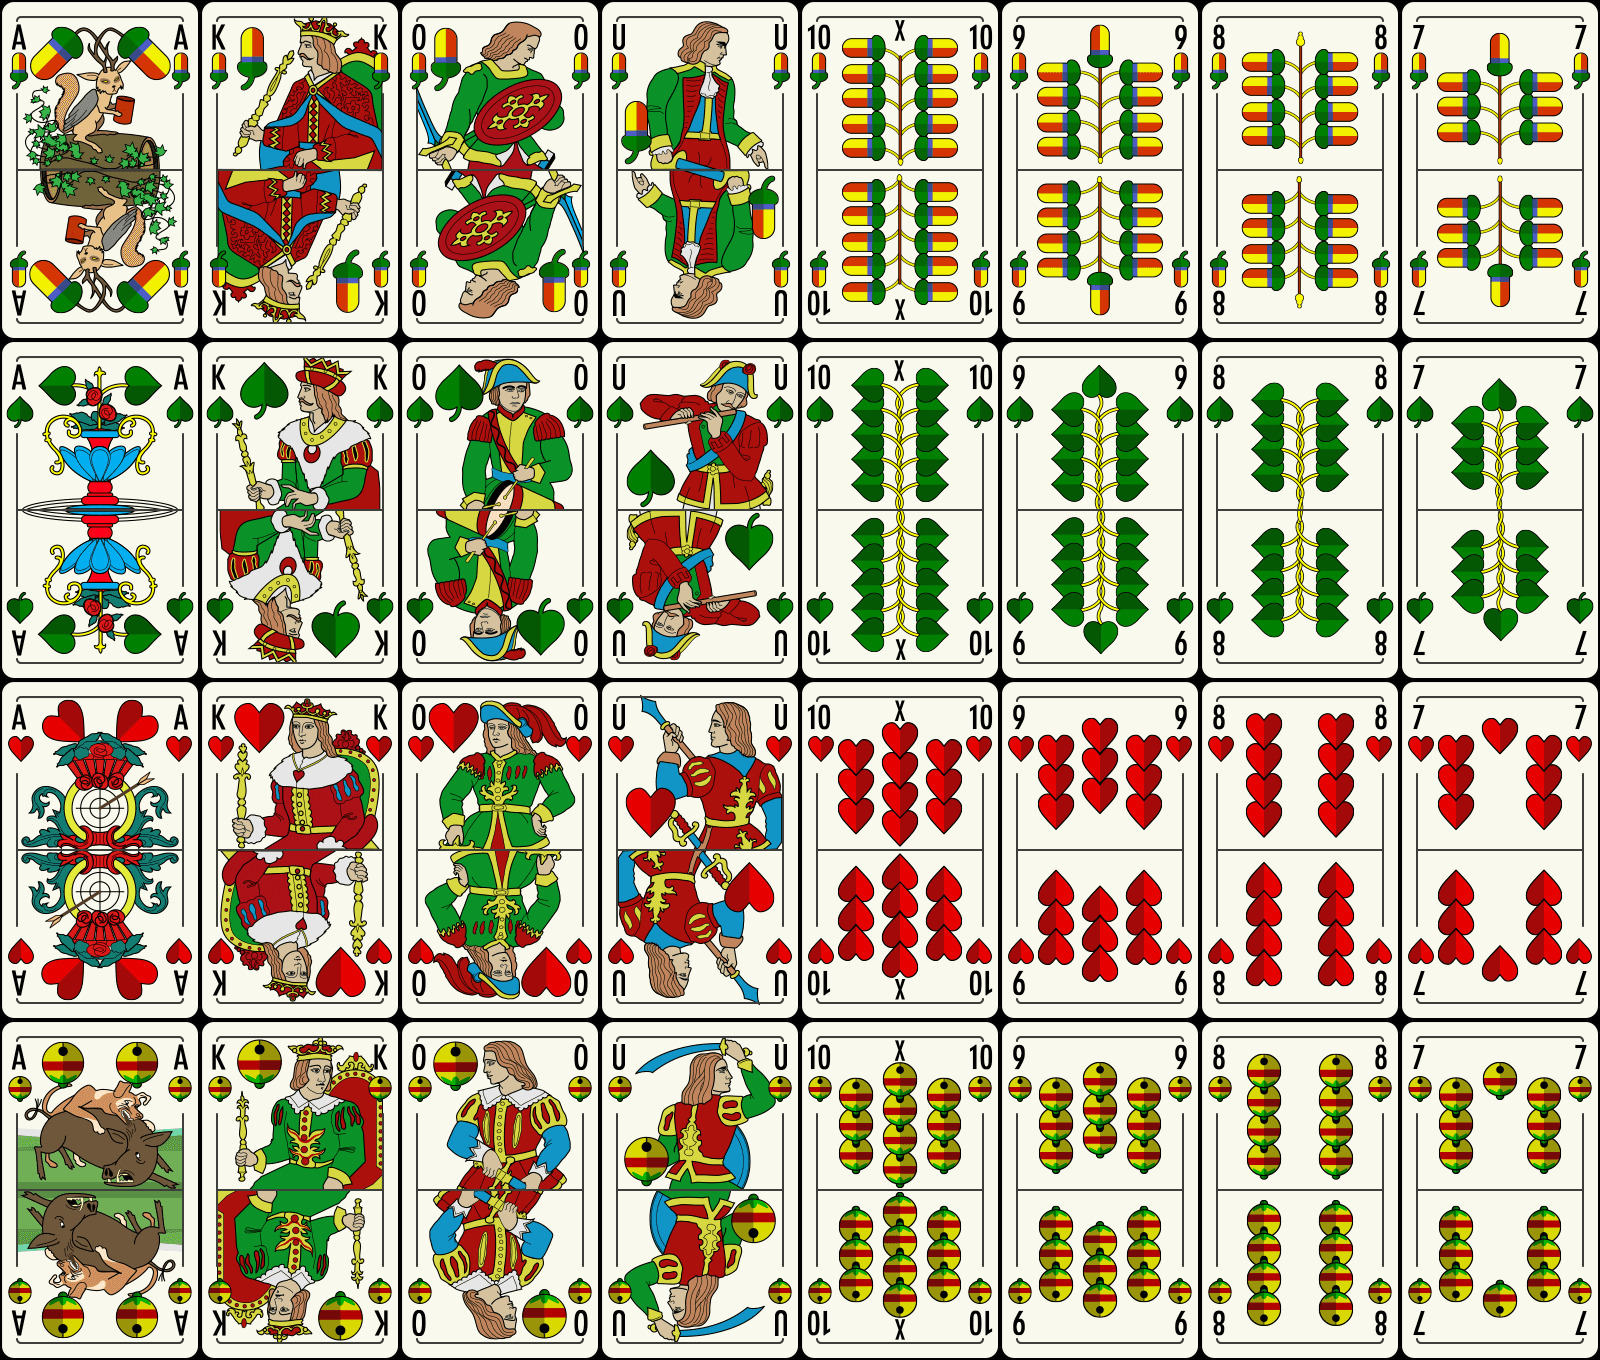
\includegraphics[scale=0.2]{cards.jpg}
    \caption{The 32 cards in Schafkopf}
    \label{fig:32cards}
\end{figure}


\section{Goal and Rules}

\subsection{Goal}
The goal is to score points by taking tricks, of which there are eight.
If a team after all cards are played has 61 points (the opposition requires only 60) the game is won.
The rules set for Schafkopf depends on the contract that is being played, there are however certain rules, such as
trick taking and following suit where possible, that always apply.

\subsection{Trumps}
Schafkopf has a set of cards that are considered trump.
This set of cards is determined by the contract that is played.
\newline
Each set has an order of strength that always follows the order of Ober > Unter > Color.
The suits themselves have also an order of Eichel > Gras > Herz > Schellen.
As an example the order of trumps for the most common contract Team, where all Ober, all Unter and all Herz are trump:
\newline
(OE,OG,OH,OS,UE,UG,UH,US,AH,TH,KH,9H,8H,7H)

\subsection{Trick}
There are two kinds of tricks, trump and suit.
The first card of each trick,which can either be of trump or a normal suit, determines which kind is present.
In both cases players behind must play a card of that suit/trump.
If they do not possess one of that kind they may play any other card, even trump if the first card played is a suit.
\newline
A suit trick can be won either by having the highest card suit on the table or by having the highest trump on the table.
Trump tricks can however only be won by playing the highest trump.
There is no obligation to win a trick if you can do so.
Other restrictions and obligations on which cards can be played will be introduced in the Team contract section,
but the above rules are sufficient in most cases.


\section{Game Phases}[\label{gamephases}]
At the beginning of each player is seated at the table, and a player is randomly chosen to deal.
The initial seating relative to one another should not be changed, since the dealer position rotates after each hand
clockwise, and if changed would skew the fairness.
\newline
Every hand of Schafkopf can be broken down in four distinct phases:
\begin{enumerate}
    \item Setup Phase
    \item Bidding Phase
    \item Trick Phase
    \item Scoring Phase
\end{enumerate}
To avoid complexity we excluded, the doubling stage (players can choose to double the final hand reward after they
receive the first half of their hand), as well as the Contra stage (opposition players may double the stakes after the
first card of the first trick is played).

\subsection{Setup Phase}
At the beginning of a hand the player in the dealer position shuffles the cards and deals each player a hand of eight
cards.
This player is called the Dealer, and the player to his immediate left is Lead and has plays the first card in the
first trick.

\subsection{Bidding Phase}
The player with the lead starts the bidding phase and can either announce Pass or Play, then the next player
clockwise announces his bid.
This continues until all players announced their intentions.
If a previous player announced Play, players may only also announce Play if they intend to choose a Solo Mode (Wenz
and Solo).
If every player passes, the hand ends, and the current dealer reshuffles the cards and returns to the Setup Phase.
If only one player announced Play, he announces his chosen contract, and the Trick Phase begins.
If more than one player announced Play, the players with the highest bid wins the bid.
The order goes TEAM < WENZ < SOLO

\subsection{Trick Phase}
The player with the Lead plays his first card, and the play continues in clockwise order until everybody played one
card.
The winner of the current trick collects all cards and becomes the new Lead.
After all eight tricks have been played the game moves into the scoring phase.

\subsection{Scoring Phase}\label{scoringphase}
Each team counts their combined points, and a winner is determined.
The team that won the bid requires 61 points, whilst the opposition team only requires 60 points.
The rewards can now be calculated using a prearranged structure.
The base value of a game depends on the contract
that is being played,where SOLO modes are rewarded more due to their higher risk.
\newline
There are also specials rewards a team can earn:
\begin{description}
    \item[Schneider] The bid winners can claim Schneider when the opposition has not scored 30 points and vice versa
    if the bid winners have not scored 31 points.
    \item[Schwarz] A winning team can claim Schwarz if the other team have not won a single trick.
    A trick with 0 points still counts as trick win.
    \item[Laufende] Laufende is a row of the highest trumps held by a party without interruption.
    In the TEAM game and COLOR Solo, payment is made from three Laufende (at least OE,OG,OH) and in the WENZ,
    payment is made from two Laufende (at leas UE,UG).
    Laufende can range from 2 up to 14 depending on which contract is played.
\end{description}
The formula to calculate the final hand reward is always:
\[\text{Hand Reward} = \text{Base Reward} + \text{Schneider} + \text{Schwarz} + \text{Laufende}\]
Losers pay the winners the Hand rewards, thus making it a zero-sum game.
In TEAM game the losers get the negative hand reward, and the winners receive the positive hand reward.
In SOLO the bid winner receives three time the reward and each player receives a single hand reward.
Traditionally players set a price to a reward, e.g. 1 reward point equals 0,01 \texteuro, which are eventually won or
lost.
Also the reward for different game modes may be set individually.
The structure used in this paper can be found in Table \ref{tab:rewardsStrucutre}.
After the scoring phase the hand is now finished, and the dealer role rotates clockwise to start a neew hand
\begin{table}[h!]
    \centering
    \begin{tabular}{cc}
        \toprule
        Game Mode & Base Reward \\
        \midrule
        Specials  & 10          \\
        Team      & 20          \\
        Solo      & 50          \\
        \bottomrule
\end{tabular}
    \caption{The standard rewards in Schafkopf}
    \label{tab:rewardsStrucutre}
\end{table}


\section{Contracts}
Schafkopf has a lot of differing contracts, these often allow for more Solo contracts or avoid aborting the hand.
All contracts follow the same trick rules we defined earlier, and only differ in the way the players are divided in
teams,what cards are Trump and the order of card ranks.
For this implementation we considered only the three classic contracts:
\begin{itemize}
    \item Team Mode
    \item Wenz
    \item Color Solo
\end{itemize}
Team mode is a two vs two variant and most, whilst WENZ and COLOR SOLO both pit the bid winner against the other three.

\subsection{Team}
In the Team game there are 14 Trumps: four Ober, four Unter and all Herz.
\newline
The bid winner calls a color ace that she does not hold herself, but she must hold at least one card of that color
that is not trump.
An example can be seen in Figure \ref{fig:bidding}
The player that holds the ace, being called the partner, will be allied for with the bid winner, whilst the remaining
players form the opposition team.
\newline
\begin{figure}[h!]
    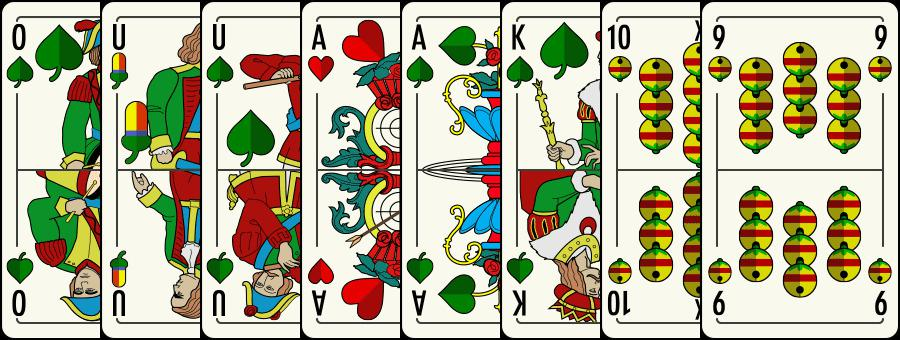
\includegraphics[scale=0.5]{partnerBiddingExample}\label{fig:figure}
    \caption{The player can only search for AS, since he holds the AG himself and has no Eichel himself}
    \label{fig:bidding}
\end{figure}
\newline
At the beginning of the hand only the partner knows the full team compositions, but in normal play this becomes
apparent fairly soon, can sometimes however last until the last trick.
If a trick starts with the searched color, the Partner has to play the ace.
This process is called Searching and reveals the team composition.
\newline
The partner may play the Ace at the beginning of a trick himself if he has the lead.
If no one searches the ace may only be played in the last trick.
If the partner has a four cards or more of the searched suit,including the ace, he may run away by playing a different
card of that suit, if and only if he has the lead.
Once runaway he may play the ace at any point.
This is due to the fact that if the partner holds 4 cards of the suit, the bid winner one, there is only one remaining
card with the opposition.
This would guarantee a lost trick if the opposition searches and holds trump.

\subsection{Solos}
The Solos, in which the bid winner plays alone against the other three players, require a much stronger hand in general
in order to win.
There is an obvious risk to this, due to not having a partner, but there is also a higher base reward for Solos.
This reward is also earned and lost from three players rather than one compared to the TEAM mode.

\subsubsection{Suit Solo}
The bid winner calls which color is trump.
As with the Team game there are 14 Trumps, four Ober, four Unter and six cards of the chosen color.
The team composition is obvious after the bid winner announces his game.

\subsubsection{Wenz Solo}
In the Wenz Solo the only trumps are the four Unter.
The Ober are now considered color and slot in after the King in terms of card ranking.


\section{Basic Strategy}
Schafkopf is a game with a lot of subtle and deep strategies that can take a many hands to master, yet most beginners
are given a set of base rules to follow.
Most of these rules are role dependent and will be outlined shortly below.

\subsection{Search and runaway when possible}
Players should always search when they have the chance.
Since at least two of the six searched suit cards are between the bid winner and her partner and one is with herself
the chance is high that her partner holds no cards of that suit and can trump.
The more cards of the suit he holds himself, the more likely it is that his partner is free on the searched suit and
can win the trick by playing trump.
Often winning this trick is a requirement for the opposition to winning the game.
Another benefit of searching is to gain information about the team composition, since the opposition knows the least
about it.\\
Due to the natural imbalance of trumps between the two teams, the opposition will most likely score fewer tricks and
thus benefit from knowing who their partner is.
This way they can use their trumps and high scoring cards more efficiently.
\newline
The searched partner in a team should always run away when he holds four suit cards in order to reduce the points lost
to the opposition.
This way he saves the 11 points of the ace for a later trick.
A rare exception to the rule is when the searched player holds 5 cards and the bid winner the last.
In this case running away is pointless since the opposition has no means of searching in the first place.
\newline
Although this rule only applies to players that have the lead, it can still be useful in other situations.
For example when players have the chance to take the lead by winning a trick only as a means to search or run away in
the following trick.
This can sometimes mean taking away a trick of the partner or winning a low scoring trick.

\subsection{Bidder plays Trump,oppositon plays color}
This rule refers to the decision when a player has the lead, and applies to both Solo and team games.
Since the bid winner announced the game he should have more trumps than the other players and thus also fewer colors.
By playing trump when he has the lead, he can drain the opposition's trumps.
After the opposition no longer holds trump, consecutive colors such as [A,T,K] gain in strength as they cannot be
trumped anymore.
If the player had played color from the beginning, the trick could have been lost.\\
In team mode this rule also applies to the searched player and often serves as a way of signaling team membership,
since playing trump and being on the opposition in general is counterproductive.
\newline
The reverse logic applies to the opposition's strategy, as they have fewer trumps they should use the lead as an
opportunity to play color to see if they can score this way as it is unlikely to make many tricks
with trump.
If a player has aces he should play them early, before the bid winner can rid himself of that color, or play a low
color in the hope that his partner holds the ace or has trump left in case he does not hold the color himself.
\newline
In team games this strategy also servers as way of signalling team membership, especially if the lead in the first
trick opens with a suit that is not the searched ace.
By not playing trump and not searching the player signals he is part of the opposition and can not search.
His partner in turn should thus try to gain the lead in order to search before the other team drains all their trumps.

\subsection{}

